
\chapter{Multi-core Communication}
\startcontents[chapters]
\printcontents[chapters]{}{1}{}

\noindent\\
So far we have discussed the features and design of the Vmicro16 system-on-chip. This section will discuss the multi-processing functionality and how to use it.

\section{Introduction}
Multi-processing functionality is the primary deliverable of this project.

\subsection{Design Goals}
\begin{itemize}
\item \textbf{Support common synchronisation primitives.}\\
Software should be able to implement common synchronisation primitives, such as mutexes, semaphores, and memory barriers, to perform atomic operations and avoid race conditions, which are critical in parallel and concurrent software applications.

\item \textbf{Context identification.}\\
The SoC should expose configuration information such as: the number of processing cores, amount of shared and scratch memory, and the \verb|CORE_ID|, to each thread.

\end{itemize}


\begin{figure}[h]
\centering
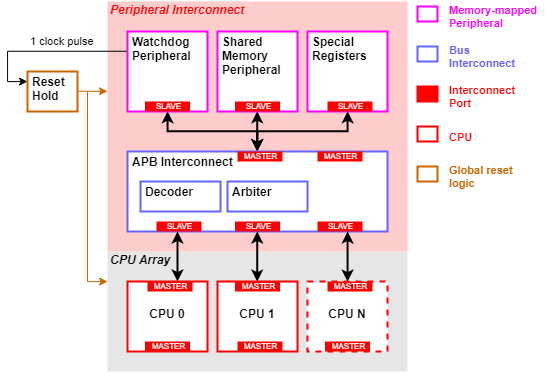
\includegraphics[width=0.7\textwidth]{multicore}
\caption{Block digram showing the main multi-processing components: the CPU array and a peripheral interconnect used for core synchronisation.}
\label{fig:multicore}
\end{figure}

\subsection{Context Identification}
A goal of the multi-processing functionality of this project is allow software written for it to be run on any number of cores. This means that a software program will scale to use all cores in the SoC without needing to rewrite the software. To enable this functionality, the software must be able to read contextual information about the SoC, such as the number of cores, how much global and scratch memory is available, and what the \verb|CORE_ID| of the current core is. 

This information is provided through the Special Registers peripheral (0x0080 - 0x008F), shown in Figure \ref{fig:multicore}. This register set provides relevant information for writing software that can dynamically scale for various SoC configurations.

\begin{figure}[H]
\centering
\begin{bytefield}[bitwidth=4ex, rightcurly=., rightcurlyspace=0pt]{16}
\bitheader[endianness=big]{0-15} \\
\begin{rightwordgroup}{0080 R}
\bitbox{8}{\color{lightgray}\rule{\width}{\height}} & \bitbox{8}{CORE\_ID}
\end{rightwordgroup} \\
\begin{rightwordgroup}{0081 R}
\bitbox{8}{\color{lightgray}\rule{\width}{\height}} & \bitbox{8}{NUM\_CORES}
\end{rightwordgroup} \\
\begin{rightwordgroup}{0082 R}
\bitbox{16}{SHARED\_MEMORY cells \tiny(default 4096)}
\end{rightwordgroup} \\
\begin{rightwordgroup}{0083 R}
\bitbox{8}{\color{lightgray}\rule{\width}{\height}} & \bitbox{8}{NUM\_PERIPHERALS}
\end{rightwordgroup} \\
\begin{rightwordgroup}{0084 RW}
\bitbox{16}{SCRATCH\_MEMORY cells \tiny(default 64)}
\end{rightwordgroup} \\
\begin{rightwordgroup}{0085 RW}
\bitbox{16}{User defined}
\end{rightwordgroup} \\
\bitbox[]{16}{$\vdots$ \\[1ex]} \\
\begin{rightwordgroup}{008F RW}
\bitbox{16}{User defined}
\end{rightwordgroup}
\end{bytefield}
\caption{Vmicro16 Special Registers layout (0x0080 - 0x008F).}
\end{figure}

\subsection{Thread Synchronisation}
In multi-threaded software it is important 

The mutex functionality is implemented using a similar scheme to that of ARM's \textit{Global Monitor} \cite{armgmonitor}.

\subsubsection{Mutexes}
In software, a mutex is an object used to control access to a shared resource. The term \textit{object} is used as it's implementation is normally platform dependant, meaning that the processor may provide a hardware mechanism or is left for the operating system to provide.

In this project, mutexes are provided by the processor through the Shared Memory Peripheral (0x1000 to 0x1FFF) which provides a large RAM-style memory accessible by all cores through the peripheral interconnect bus. This large memory is explicitly defined to use the FPGA's BRAM blocks using Xilinx's Verilog \verb|ram_style="block"| attribute to avoid wasting LUTs when using high core counts. The peripheral allows each memory cell to be \textit{locked}, meaning that only the cell owner can modify it's contents. This is implemented by using another large memory, \verb|locks|, to store the $\verb|CORE_ID| + 1$ of the owner, as shown in Figure \ref{fig:lock}. In this system, a lock containing the value zero indicates an unlocked cell. As \verb|CORE_ID|s are indexed from zero, one is added to each cell. For example, if core two wants to lock a memory cell, the value three is written to the lock.

\begin{figure}[h]
\centering
\begin{minted}{verilog}
reg [15:0]           ram   [0:8191]; // 16KB large RAM memory
reg [clog2(CORES):0] locks [0:8181]; // memory cell owner
\end{minted}
\caption{RAM and lock memories instantiated by the shared memory peripheral.}
\label{fig:lock}
\end{figure}

To lock and unlock cells, the instructions \verb|LWEX| and \verb|SWEX| instructions are used. These instructions are similar to the \verb|LW/SW| instructions but provide locking functionality. The \textit{EX} in the instruction names indicate \textit{exclusive access}. \verb|LWEX| is used to read memory contents  (like \verb|LW|) and also lock the cell if not already locked. If a core attempts to lock an already locked cell, the lock does not change. Unlocking is done by the \verb|SWEX| instruction, which conditionally writes to the memory cell if it is locked by the same core. Unlike \verb|SW|, \verb|SWEX| returns a zero for success and one for failure if it is locked by another core.

\begin{wrapfigure}{L}{0.5\textwidth}
\centering
\begin{minted}[fontsize=\footnotesize,
    baselinestretch=0.8,]{arm}
lock_mutex:
	// attempt lock
	lwex r0, r1
	// check success
	swex r0, r1
	cmp  r0, r3
	// if not equal (NE), retry
	movi r4, lock_mutex
	br   r4, BR_NE
critical:
    // core has the mutex
\end{minted}
\caption{Assembly code for locking a mutex. r1 is the address to lock. r3 is zero. r4 is the branch address.}
\label{fig:codemutex}
\end{wrapfigure}

Figure \ref{fig:codemutex} shows a simple assembly function to lock a memory cell.

\if 0
\begin{figure}[h]
\centering
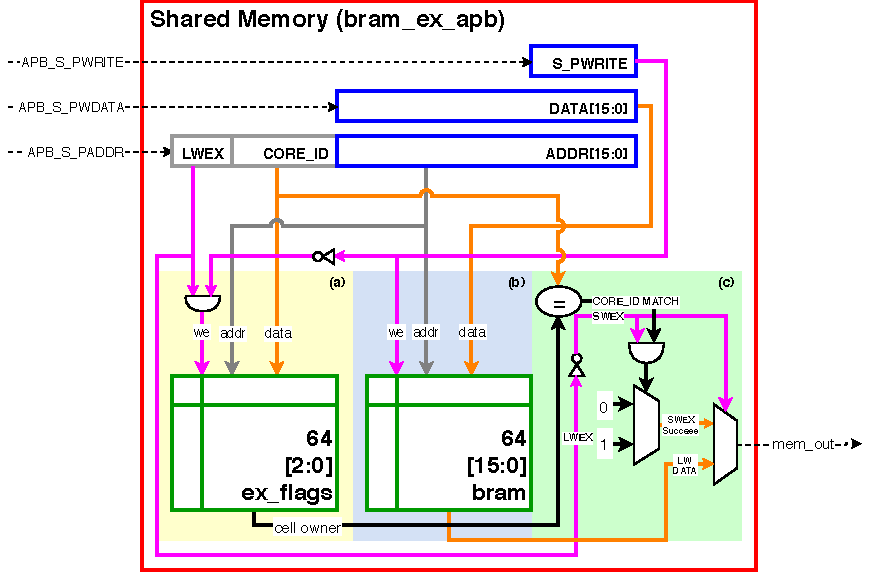
\includegraphics[width=\textwidth]{bram_ex}
\caption{Shared Memory Peripheral schematic showing RAM memory and lock memories.}
\label{fig:bram_ex}
\end{figure}
\fi


\subsubsection{Barriers}
Barriers are a useful software sequence used to block execution until all other threads (or a subset) have reached the same point. Barriers are often used for broadcast and gather actions (sending values to each core or receiving them). They are also used to synchronise program execution if some threads have more work to do than others.

\begin{wrapfigure}{L}{0.5\textwidth}
\centering
\begin{minted}[fontsize=\footnotesize,
    baselinestretch=0.8,]{arm}
barrier_reached:
    // load latest count
    lwex    r0, r5
    // try increment count
    // increment by 1
    addi    r0, r3 + #0x01
    // attempt store
    swex    r0, r5

    // check success (== 0)
    cmp     r0, r3
    // branch if failed
    movi    r4, barrier_reached
    br      r4, BR_NE

barrier_wait:
    // load the count
    lw      r0, r5
    // compare with number of threads
    cmp     r0, r7
    // jump back to barrier if not equal
    movi    r4, barrier_wait
    br      r4, BR_NE
\end{minted}
\caption{Assembly code for a memory barrier. Threads will wait in the barrier\_wait function until all other threads have reached that code point.}
\label{fig:codebarrier}
\end{wrapfigure}

The Vmicro16 processor provides barrier synchronisation through the Shared Memory Peripheral. Like the mutex code, the barrier code uses the \verb|LWEX| and \verb|SWEX| instructions to lock a memory cell. Instead of immediately checking the lock as an abstract object, the barrier code treats the cell as a normal memory cell containing a numeric value. Figure \ref{fig:codebarrier} shows a software example of this. When the \verb|barrier_reached| code is reached, the code will increment the shared memory value by 1, indicating that the number of threads that have reached this point has increased by one (r5). The \verb|barrier_wait| function is then entered which waits until this numeric value (r5) is equal to the number of threads (r7) in the system. If this is true, then all threads have reached the \verb|barrier_wait| function and can continue with normal program execution.

\section{Design Challenges}
\subsection{Memory Constraints}


\begin{figure}[H]
\centering
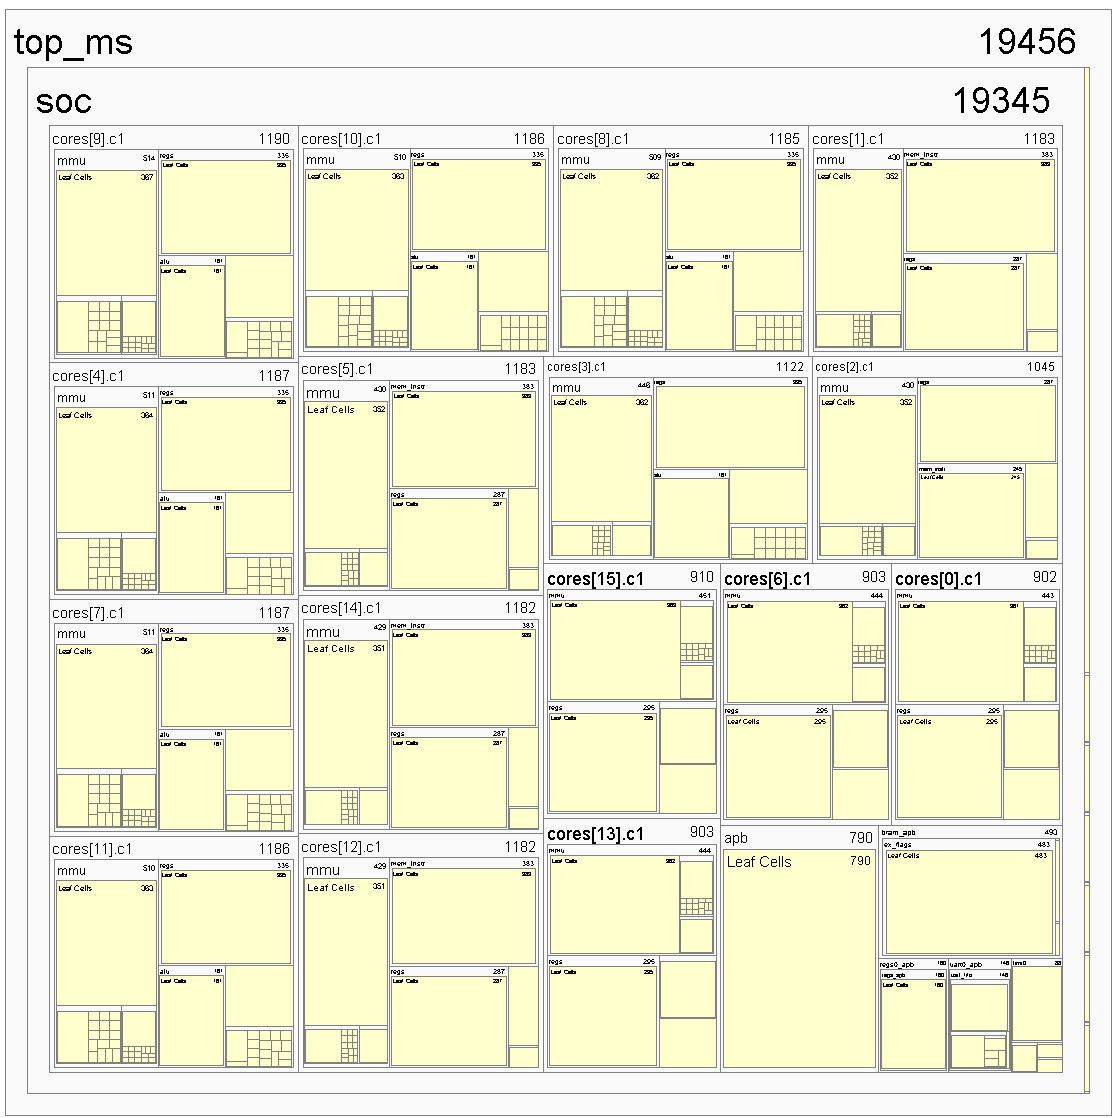
\includegraphics[width=13cm]{soc_layout_schem}
\caption{•}
\label{}
\end{figure}